\chapter{Evaluation\label{evaluation}}

This chapter discusses how the changes implemented in chapter \ref{improvements} impact the performance of RIR.

For evaluation, the Shootout benchmarks were used (see \autocite{fastr, shootout}). These are small programs that focus on different parts of R, such as recursive calls, loops, vector arithmetic, string manipulation etc. The details are in table \ref{tab:shootout}, taken from \autocite{fastr}.

\begin{longtable}[c]{@{}ll@{}}
\caption{The Shootout benchmark suite\label{tab:shootout}} \tabularnewline
\toprule
Benchmark & Description \tabularnewline
\midrule
\endfirsthead
\toprule
Benchmark & Description \tabularnewline
\midrule
\endhead
binarytrees & Allocates and traverses binary trees \tabularnewline
& \emph{GC benchmark, recursive calls, recursive lists} \tabularnewline
fannkuchred & Solves a combinatorial problem \tabularnewline
& \emph{Loops, indexing short vectors} \tabularnewline
fasta & Generates DNA sequence by copying, rand. selection \tabularnewline
& \emph{String operations, scalar arithmetic} \tabularnewline
fastaredux & Solves same problem as fasta \tabularnewline
& \emph{Adds more loops, vector indexing and arithmetic} \tabularnewline
knucleotide & Finding patterns in gene sequences \tabularnewline
& \emph{Uses environment as a hashmap, string operations} \tabularnewline
mandelbrot & Calculates a Mandelbrot set (fractal image) \tabularnewline
& \emph{Vector arithmetic on complex numbers} \tabularnewline
nbody & Solves the N-body problem (simulation) \tabularnewline
& \emph{Arithmetic, Math with short vectors} \tabularnewline
pidigits & Calculate digits of pi using spigot algorithm \tabularnewline
& \emph{Arbitrary precision arithmetic in R (diverse code)} \tabularnewline
regexdna & Matching, replacing regex-specified gene sequences \tabularnewline
& \emph{Regular expressions (falls back to regex library)} \tabularnewline
reversecompl & Computing reverse-complements for gene sequence \tabularnewline
& \emph{String vector indexing using string names} \tabularnewline
spectralnorm & Computing eigenvalue using power method \tabularnewline
& \emph{Loops, function calls, scalar arithmetic} \tabularnewline
\bottomrule
\end{longtable}

The benchmarks were run on a machine with \emph{Intel(R) Core(TM) i5-6500} (4 cores) and 8~GB of memory. For every benchmark, three experiments were measured: GNU R interpreted code (JIT set to 0), GNU R byte-compiled code (JIT set to 2 and optimize to 2) and RIR compiled code (JIT set to 2).

Each experiment took place in a fresh R session. The benchmark code was sourced, then it was executed 12 times, and the last 8 measured times were logged. This ensured that the machine was warmed up properly Any compile time overheads were disregarded. The same measurements were performed for every set of added features.

Figure \ref{fig:overall} shows the summary of how much the difference between RIR and GNU R was lowered for each benchmark, as well as an overall average (smaller values are better).

\begin{figure}[htbp]
  \caption{\label{fig:overall}Overview of the slowdowns vs. GNU R}
  \centering
  \tmpframe{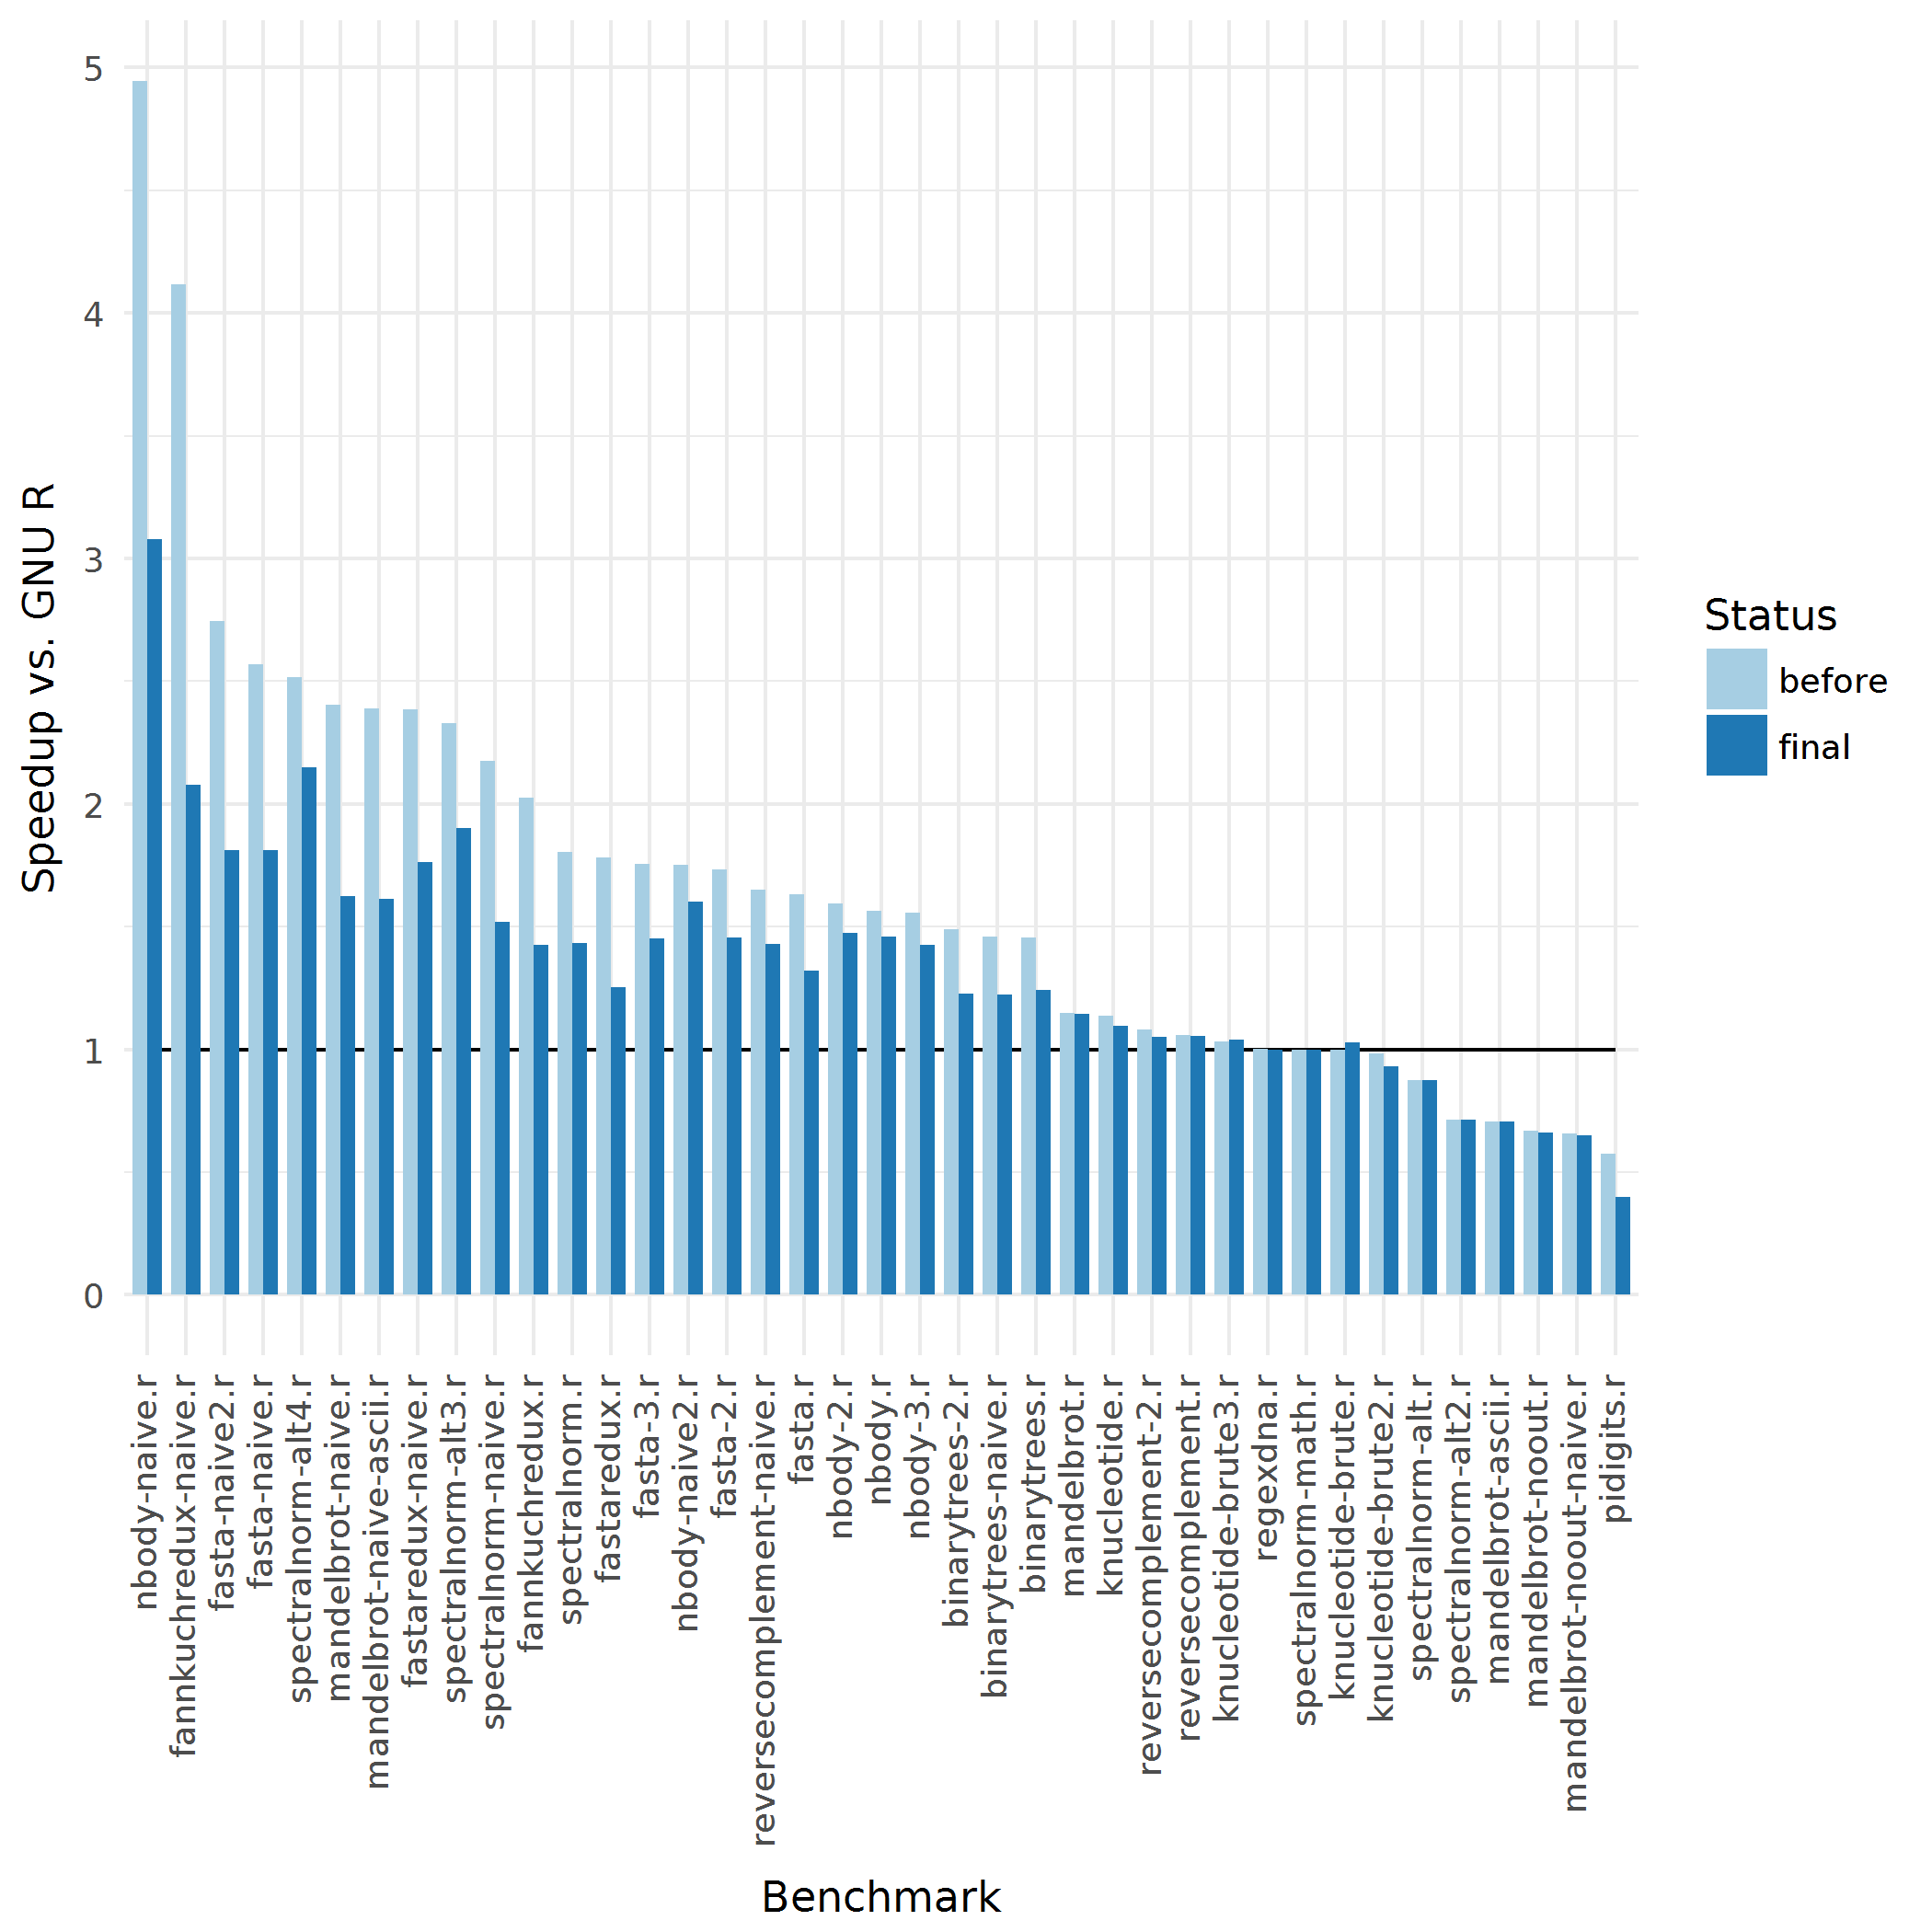
\includegraphics[width=\linewidth]{images/overall}}
\end{figure}

The lighter color refers to the state before any feature was added, the darker after all the changes described in chapter \ref{improvements}.

The slowdowns are computed relative to the running time of GNU R byte-compiled code, which was normalized to 1 (and is indicated by the solid black line).

Overall, an average slowdown against GNU R was lowered by about 50~\% (from a factor of 1.678 to 1.336).

It can be clearly seen that the most speedup was gained for the naive versions of benchmarks. These are the programs that use a lot of nested loops, lot of arithmetic operations and have relatively long functions.

\todo[more]

The revisions that were used to monitor the progress, together with their features, are listed in table \ref{tab:git-rev}.

\begin{longtable}[c]{@{}ll@{}}
\caption{Git revisions used in the benchmarks\label{tab:git-rev}} \tabularnewline
\toprule
Hash & Features \tabularnewline
\midrule
\endfirsthead
\toprule
Hash & Features \tabularnewline
\midrule
\endhead
e1091b9 & State before the first changes \tabularnewline
594af0c & Added relational and unary operators \tabularnewline
ce30085 & Loop contexts removal \tabularnewline
6c4f526 & BC cleanup and colon operator \tabularnewline
f8e8238 & Superassignment operator \tabularnewline
12ef757 & Interpreter loop refactoring \tabularnewline
ff73d75 & Use indirect threading \tabularnewline
\bottomrule
\end{longtable}

Figure \ref{fig:history} captures the running times of each benchmark over the course of the work described in chapter \ref{improvements}.

\begin{figure}[htbp]
  \caption{\label{fig:history}History of running times}
  \centering
  \tmpframe{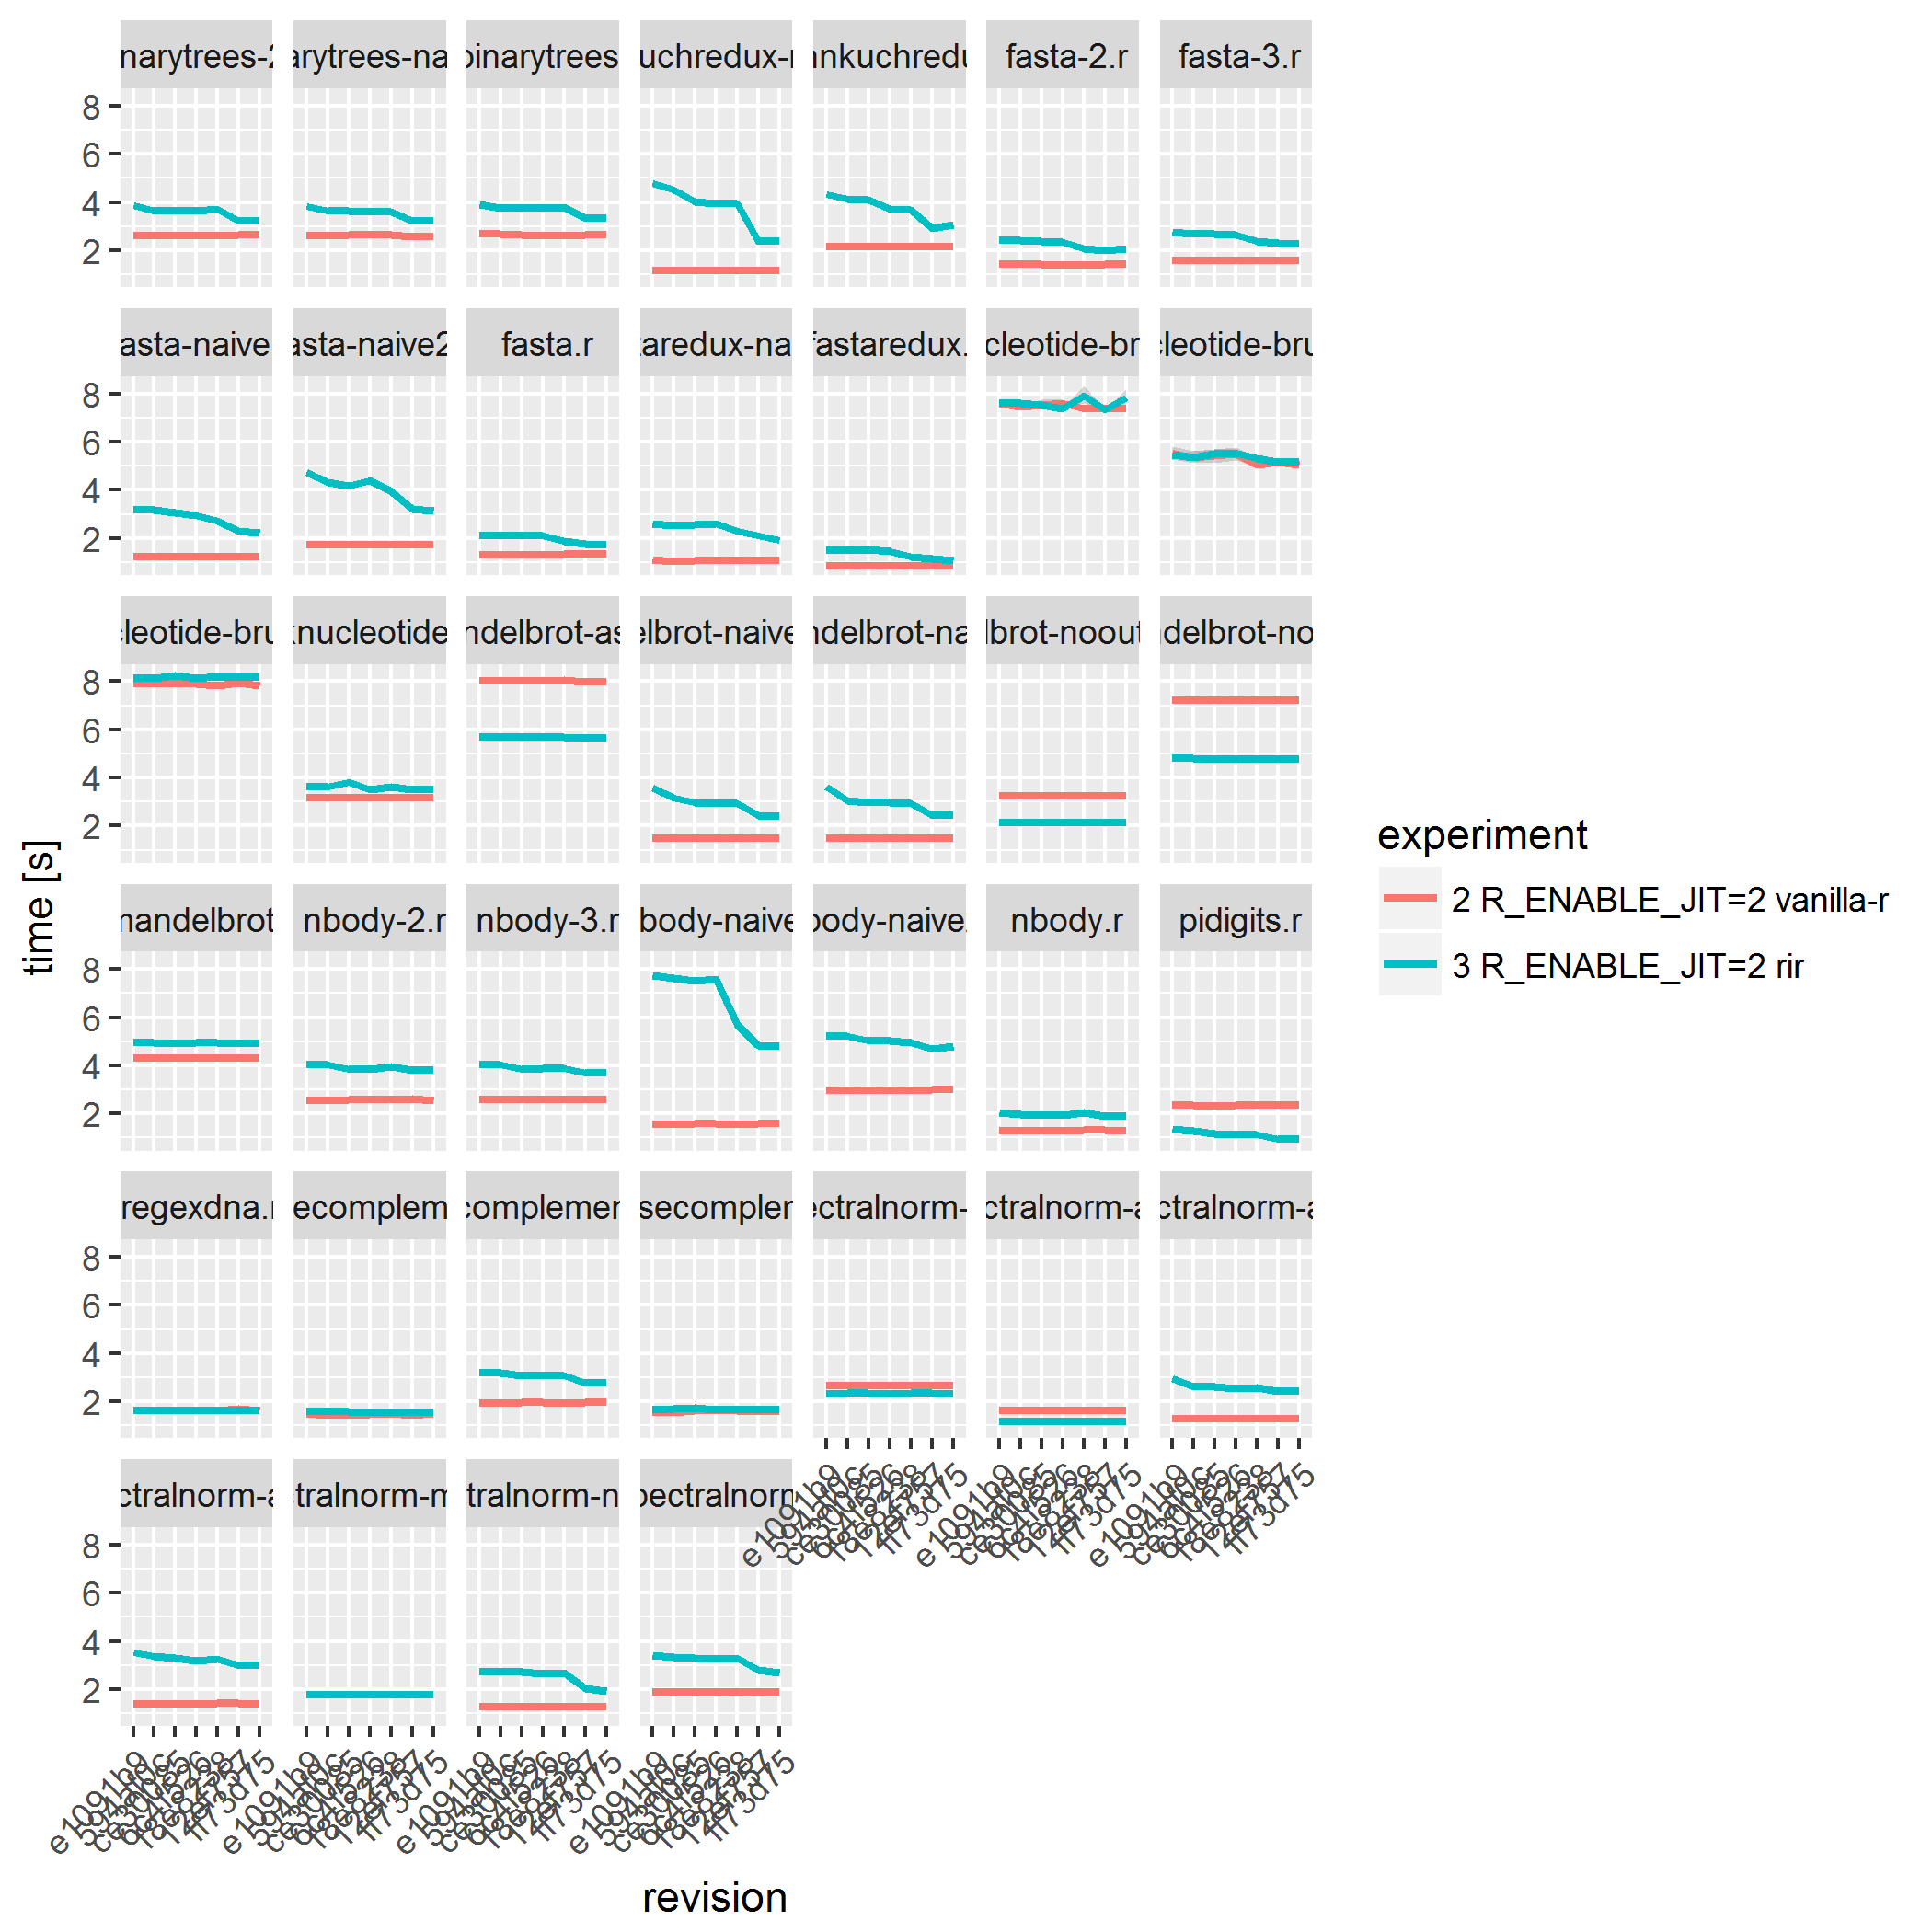
\includegraphics[width=\linewidth]{images/speedup_history}}
\end{figure}

In the figure, the light blue color represents performance of the GNU R bytecode. As all measurements were carried out on the same version of GNU R (namely 3.3.2) the times are identical.

RIR performance for some benchmarks was comparable to GNU R even before the first modifications, with some (notably \emph{pidigits}) outperforming GNU R.

Generally, the biggest improvements were brought by inlining the instructions into the interpreter loop. With the exception of some benchmarks not effected by any changes, all others gained a boost.

For some benchmarks, a particular revision brings minor slowdowns. This is the case for the removal of loop contexts (\emph{knucleotide}), colon (\emph{fasta naive 2}), superassignment and threading (\emph{knucleotide brute}).

Other benchmarks (e.g., \emph{mandelbrot}, \emph{regexdna}, \emph{spectralnorm}, \emph{reversecomplement} have remained constant throughout.

The plot for \emph{nbody naive} is zoomed in in figure \ref{fig:nbody}. The benchmark gained the most with inlining superassignment, as it uses it heavily in nested loops. Another large speedup was due to the interpreter refactoring and is so distinctive because the produced bytecode for the main hotspot (the function \rinline/advance/) is very arithmetic heavy with a lot of loops and subsetting and few calls. This means that long sequences of instructions get executed at once, thus leveraging the improved interpreter loop.

\begin{figure}[htbp]
  \caption{\label{fig:nbody}Detail of the \emph{nbody naive} benchmark}
  \centering
  \tmpframe{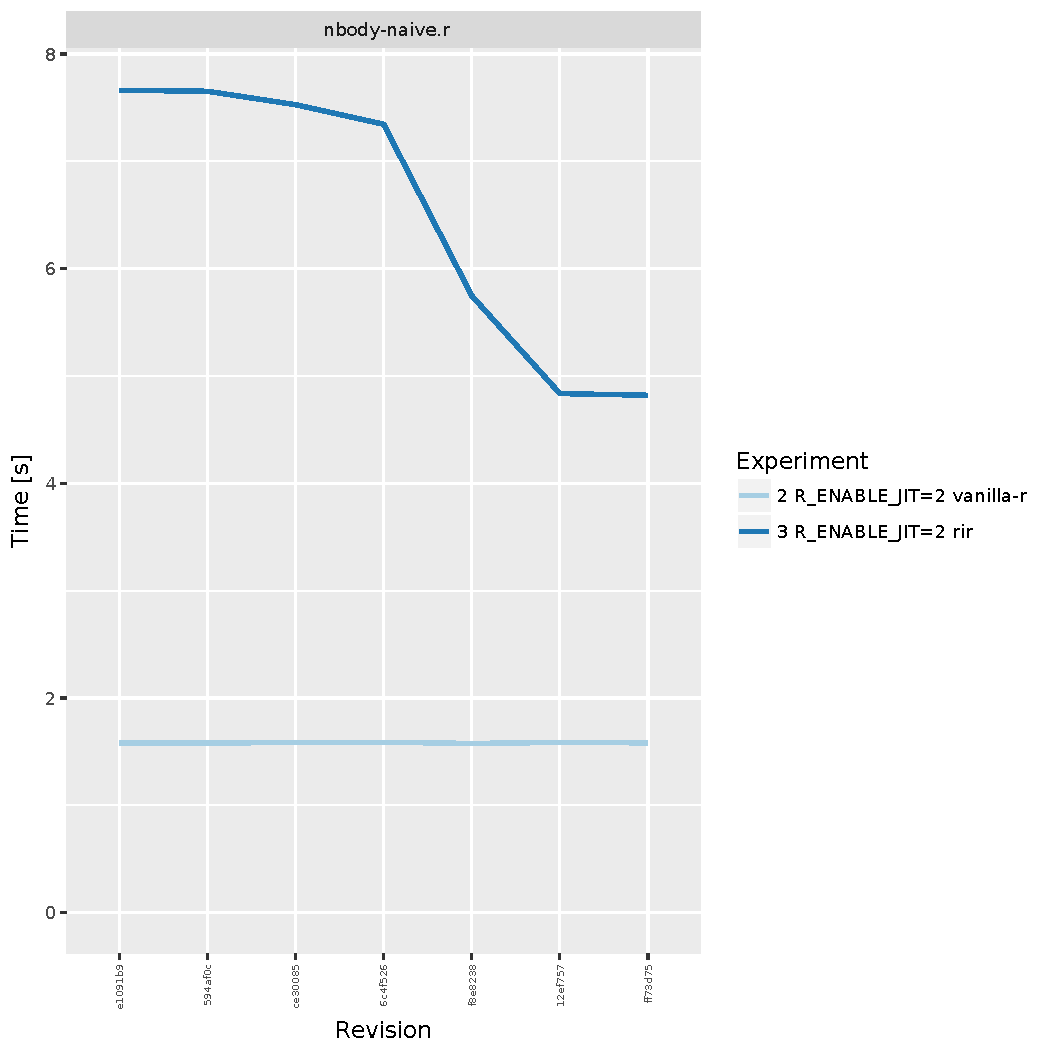
\includegraphics[width=\linewidth]{images/nbody-naive}}
\end{figure}

Another interesting result is the \emph{knucleotide brute} benchmark. Here it seems that the superassignment as well as threading made things worse. However, it also shows very wide confidence intervals.

\begin{figure}[htbp]
  \caption{\label{fig:knucleotide}Detail of the \emph{knucleotide brute} benchmark}
  \centering
  \tmpframe{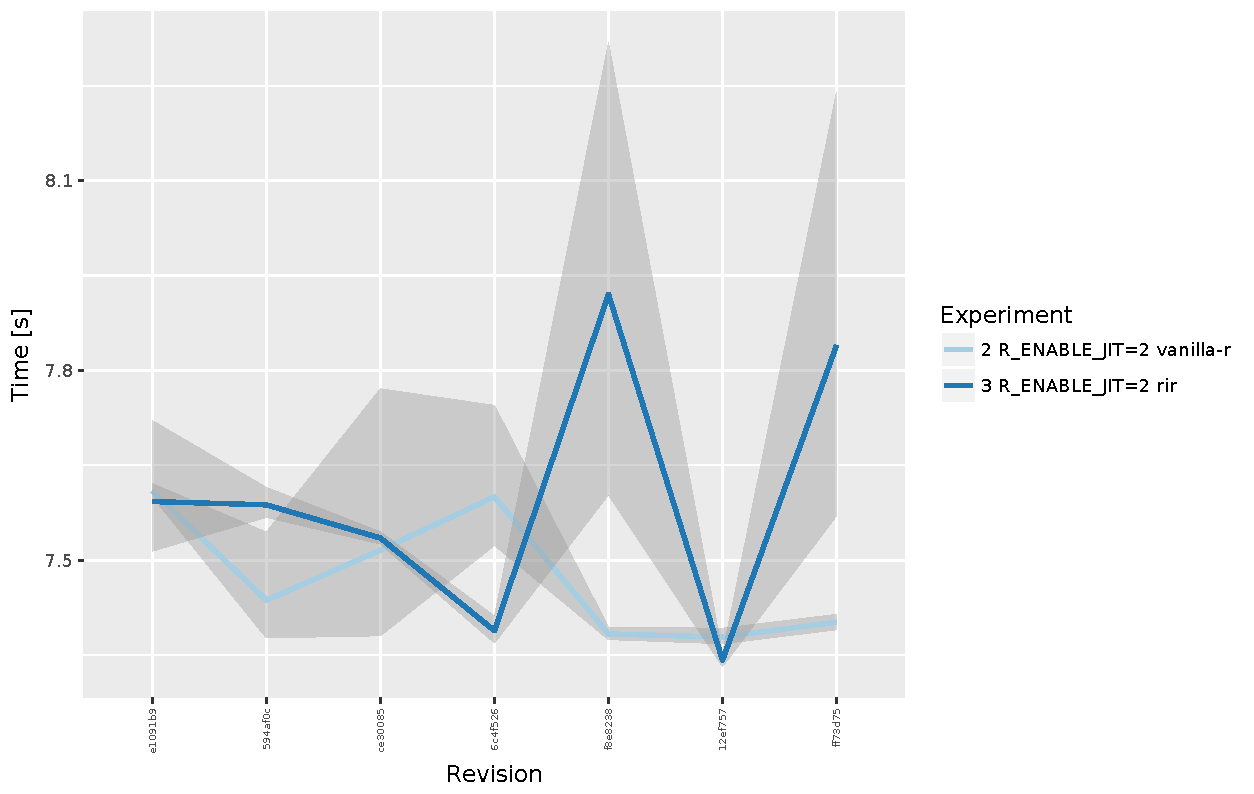
\includegraphics[width=\linewidth]{images/knucleotide-brute}}
\end{figure}

The average speedup versus GNU R over the measured revisions is captured in figure \ref{fig:avg-speedup-history}. The result was obtained by averaging the measurements for each benchmark and then taking the average of those values. From the changes, the most debatable is threading. It seems that this feature only starts to pay off for larger and longer programs.

\begin{figure}[htbp]
  \caption{\label{fig:avg-speedup-history}History of average speedup vs. GNU R}
  \centering
  \tmpframe{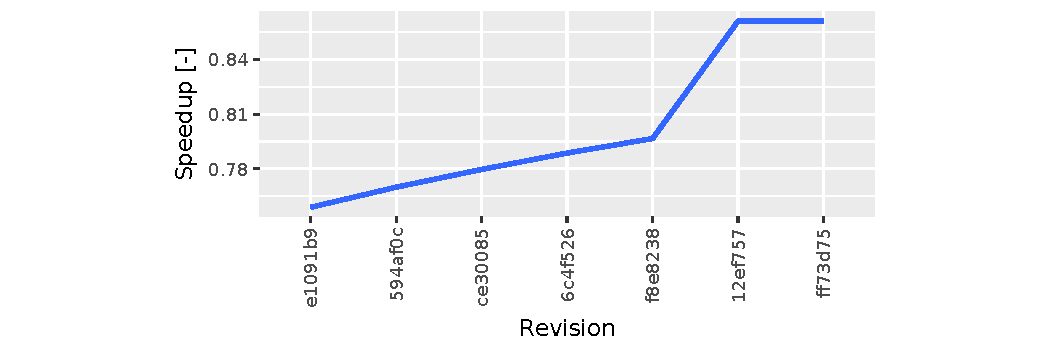
\includegraphics[width=\linewidth]{images/avg_speedup}}
\end{figure}
